\documentclass[10pt]{article}
\usepackage[a4paper,landscape,margin=0.72in]{geometry}
\usepackage[T1]{fontenc}
\usepackage{lmodern,amsmath,amssymb,graphicx,hyperref}
\title{Global principal-divisor and Picard-class proof boundary}
\author{Read-only formal dependency inventory}
\date{28 October 2026}
\begin{document}
\maketitle
\noindent Inspected isolated commit \texttt{f0c4308b62fa6a2621637d7fd02a13a148881ed4}. This packet adds no Lean theorem, experiment, target result, or cost ratio. Existing declarations are reported only with their stated hypotheses; the inventory did not rebuild all predecessors.

\section*{Checked components present}
\begin{itemize}
\item \texttt{smooth}: actual weighted-$\operatorname{Proj}$ structure map smooth over a perfect field when $2\ne0$ and the quintic is squarefree. \texttt{weightedProj\_proper\_over\_K}: properness over $K$. Full declaration names are in the CSV.
\item \texttt{source\_curve\_eq}: source-style polynomial norm under valid input congruences and nonzero determinant. \texttt{returned\_v\_cleared}: output-ordinate polynomial congruence. Full declaration names are in the CSV.
\item \texttt{WeightedProjNonbranchNormTransport}: source-style norm in an actual rational-point stalk; chosen-factor order with explicit separability, point, nonunit, $2y\ne0$, $b\ne0$, and norm premises. The separate branch theorem gives rational simple-branch order with an explicit support-root premise.
\item \texttt{WeightedProjInfinityDVR.projectiveZ\_order\_two}: local infinity order. \texttt{Common22FractionPole}: pole-five/six implications only for a supplied valuation and cleared interpolant conditions.
\item \texttt{ProjectiveLawRuntime.residual\_represents\_input}: abstract class implication only after a curve-specific principal-divisor interface and principal premise are supplied.
\end{itemize}

\section*{Open theorem boundary}
Define the actual curve function $g=n/b-Y$ and effective divisors for the two input Mumford pairs and residual pair. A global proof must show that the local orders at \emph{all closed points} (including nonrational points, branch overlap, repeated roots, and the $c=0$ degree drop) and the infinity pole determine $\operatorname{div}(g)$. It must identify this divisor as principal, match the residual divisor with the returned pair and its involution, and construct the concrete degree-zero class map. The schematic equation $\operatorname{div}(g)=D_1+D_2+Z_{\rm res}-m\infty$ is a proposed target, not a checked theorem; $m$ needs a proof by degree branch. A ring Picard group in pinned Mathlib is not already a curve-specific divisor-class construction. The abstract group implication alone cannot discharge the principal premise.

\noindent Sources: repository declarations listed in the accompanying Markdown/CSV; Stacks Project Tags \href{https://stacks.math.columbia.edu/tag/02RS}{02RS} (principal divisors) and \href{https://stacks.math.columbia.edu/tag/03RN}{03RN} (Picard groups of curves). These sources inform obligations; they do not certify the missing Lean bridge.

\clearpage
\section*{Proof dependencies}
\begin{center}
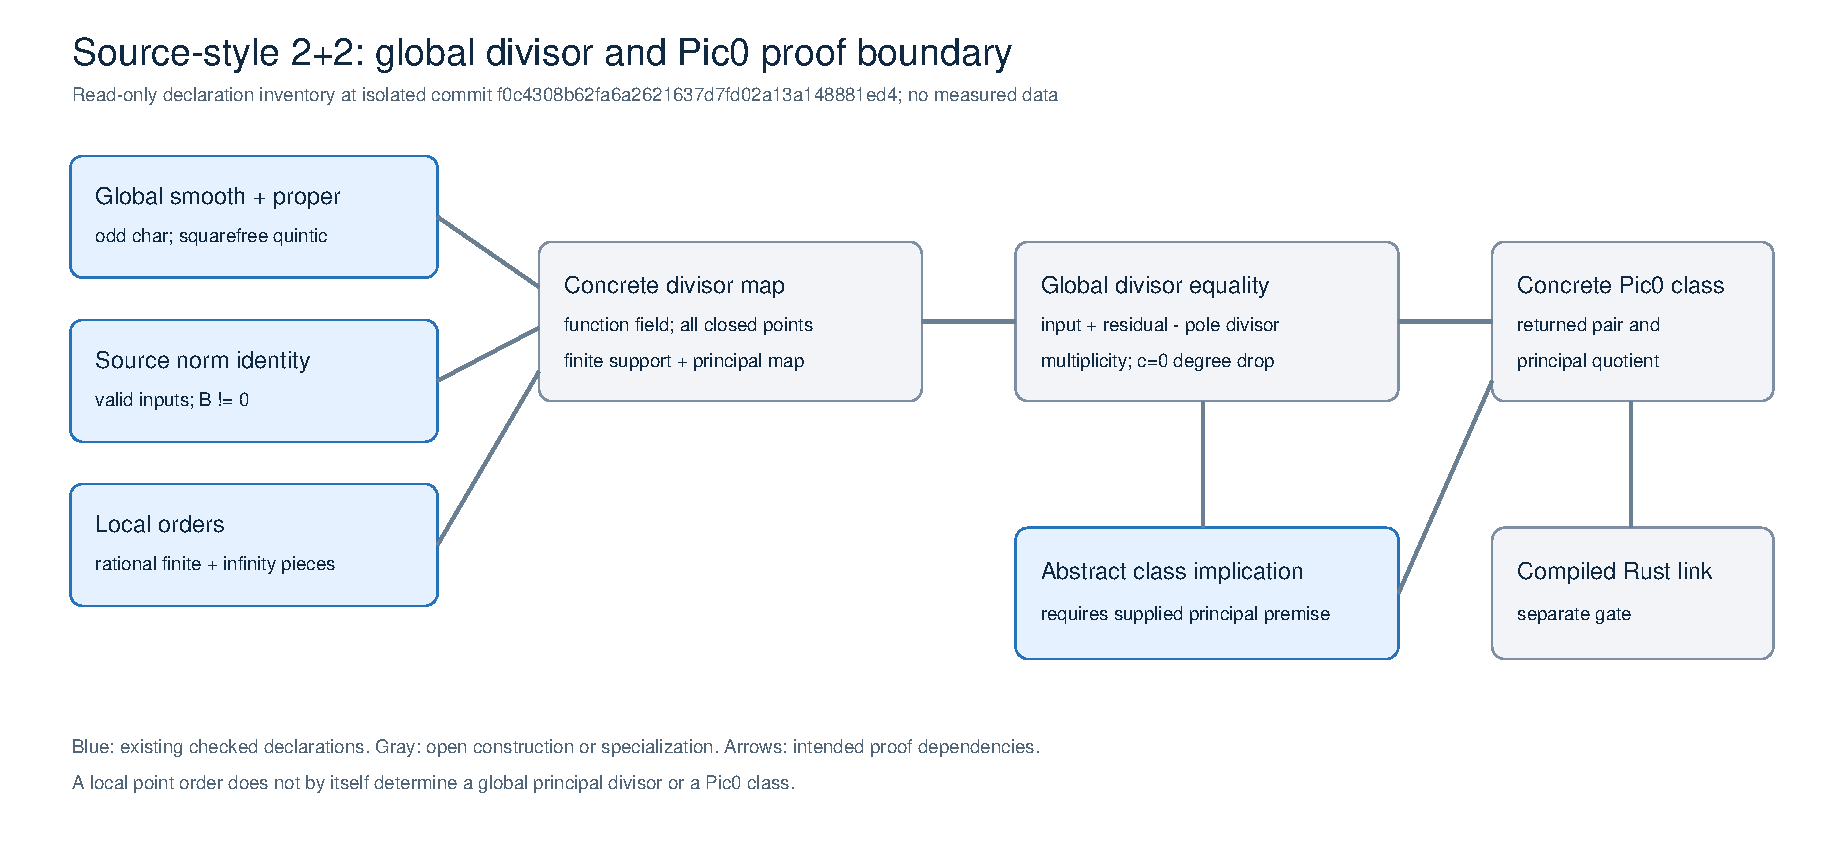
\includegraphics[width=0.96\textwidth,height=0.78\textheight,keepaspectratio]{global-pic0-gap-figure.pdf}
\end{center}
\noindent Blue boxes are existing checked declarations; gray boxes are open construction or specialization gates. Arrows show intended dependencies, not measured performance.
\end{document}
